\documentclass{beamer}
\usetheme{Copenhagen}
\usecolortheme{whale}
\usefonttheme[onlymath]{serif}

\usepackage{amsmath}
\usepackage{setspace}
\usepackage{xcolor}
\usepackage{graphicx}
\usepackage{multimedia}
\usepackage{fontawesome}
\usepackage{tikz}
\usetikzlibrary{positioning, calc, shapes.geometric, shapes.multipart, 
	shapes, arrows.meta, arrows, 
	decorations.markings, external, trees}
\tikzstyle{Arrow} = [
thick, 
decoration={
	markings,
	mark=at position 1 with {
		\arrow[thick]{latex}
	}
}, 
shorten >= 3pt, preaction = {decorate}
]

\newcommand{\blue}[1]{\textcolor{blue}{#1}}
\newcommand{\red}[1]{\textcolor{red}{#1}}
\newcommand{\violet}[1]{\textcolor{violet}{#1}}
\definecolor{ForestGreen}{RGB}{0,150,0}
\newcommand{\green}[1]{\textcolor{ForestGreen}{#1}}


\title{M-estimation for fusion designs}
\author[Paul Zivich]{Paul Zivich \\~\\ Department of Epidemiology \\ Causal Inference Research Laboratory \\ UNC Gillings School of Global Public Health}


\setbeamercovered{transparent}
\setbeamertemplate{navigation symbols}{}  % gets rid of the dumb navigation symbols
\setbeamertemplate{page number in head/foot}{\insertframenumber}  % adds slide #
\setbeamertemplate{headline}{}

\AtBeginSection[]{
	\begin{frame}
		\vfill
		\centering
		\begin{beamercolorbox}[sep=8pt,center,shadow=true,rounded=true]{title}
			\usebeamerfont{title}\insertsectionhead\par%
		\end{beamercolorbox}
		\vfill
	\end{frame}
}

\begin{document}
	\begin{frame}[plain]
		\maketitle
\end{frame}

\begin{frame}{Acknowledgements}
	Supported by NIH T32-AI007001.\\~\\~\\
	
	Thanks to Stephen Cole, Jessie Edwards, Bonnie Shook-Sa, and others at the UNC Causal Lab (causal.unc.edu).\footnote[frame]{Footnotes are reserved asides for possible later discussion or questions}\\~\\~\\~\\
	\begin{center}
		\faEnvelope \quad pzivich@unc.edu \qquad
		\faTwitter \quad @PausalZ \qquad
		\faGithub \quad pzivich\\
	\end{center}
\end{frame}

\section{M-estimation}

\begin{frame}{M-estimation\footnote[frame]{For a general introduction see either Chapter 7 of \textit{Essential Statistical Inference} or Stefanski \& Boos (2002) \textit{Am Stat}}}
	M-estimators are the solution to
	\[\frac{1}{n} \sum_{i=1}^{n} \psi(O_i; \hat{\theta}) = 0\]~\\~\\
	Estimating function for the mean
	\[\frac{1}{n} \sum_{i=1}^{n} Y_i = \mu \;\;\;\;\;\; \rightarrow \;\;\;\;\;\;\; \frac{1}{n} \sum_{i=1}^{n} (Y_i - \mu) = 0\]
\end{frame}

%\begin{frame}{M-estimation}
%	Two main advantages for estimation with fusion designs\footnote[frame]{Other commonly discussed advantages of M-estimation include the unification of large sample methods, generalization of maximum likelihood, and simplification of consistency and asymptotic normality proofs}
%	\begin{itemize}
%		\item[1.] Stack estimating function together
%		\item[2.] Automation of the procedure
%	\end{itemize}
%\end{frame}

\begin{frame}{Stacked functions}
	Example: inverse probability of missingness weighted mean
	\begin{itemize}
		\item MNAR conditional on $W$ 
	\end{itemize}
	\[\psi(O_i, \theta) = 
	\begin{bmatrix}
		\left(R_i - \text{expit}(W_i^T \beta)\right) W_i & \\
		Y_i R_i \frac{1}{\text{expit}(W_i^T \beta)} - \mu & 
	\end{bmatrix}\]~\\
	Variance of $\mu$ can be estimated via sandwich variance
	\begin{itemize}
		\item Uncertainty of $\mu$ depends uncertainty of $\beta$
	\end{itemize}
\end{frame}

\begin{frame}{Automation\footnote[frame]{delicatessen: Zivich et al. (2022) \textit{arXiv}}\textsuperscript{,}\footnote[frame]{geex: Saul \& Hudgens (2020) \textit{J Stat Softw}}}
	\centering
	\includegraphics[scale=0.75]{images/software.png}	
\end{frame}

\section{Fusion applications}

\begin{frame}{A1: measurement error\footnote[frame]{Example based on Cole et al. \textit{Am J Epidemiol} in-press}}
	Estimate mean of variable $Y$ for population $S=1$
	\begin{center}
		\includegraphics[scale=0.55]{images/data_a1.png}
	\end{center}
\end{frame}

\begin{frame}{A1: measurement error}
	Estimating functions\footnote[frame]{Measurement correction from Rogan \& Gladen (1978) \textit{Am J Epidemiol}}
	\[\psi(O_i; \theta) = 
	\begin{bmatrix}
		\green{I(S_i = 2) Y_i (Y_i^* - \alpha_1)} & \\
		\green{I(S_i = 2) (1-Y_i) (\left(1-Y_i^*) - \alpha_0\right)} & \\
		\blue{I(S_i = 1) (Y_i^* - \omega)} & \\
		\mu(\green{\alpha_1} + \green{\alpha_0} - 1) - (\blue{\omega} + \green{\alpha_0} - 1)		
	\end{bmatrix}\]~\\
	where $O_i = (S_i, Y_i, Y_i^*)$ and $\theta = (\green{\alpha_1}, \green{\alpha_0}, \blue{\omega}, \mu)$
\end{frame}

\begin{frame}{A1: measurement error\footnote[frame]{Details and code available at github.com/pzivich/Presentations}\textsuperscript{,}\footnote[frame]{Based on 2000 repetitions with $n_1=750$, $n_2=200$, and $\mu=0.37$}}
	\centering 
	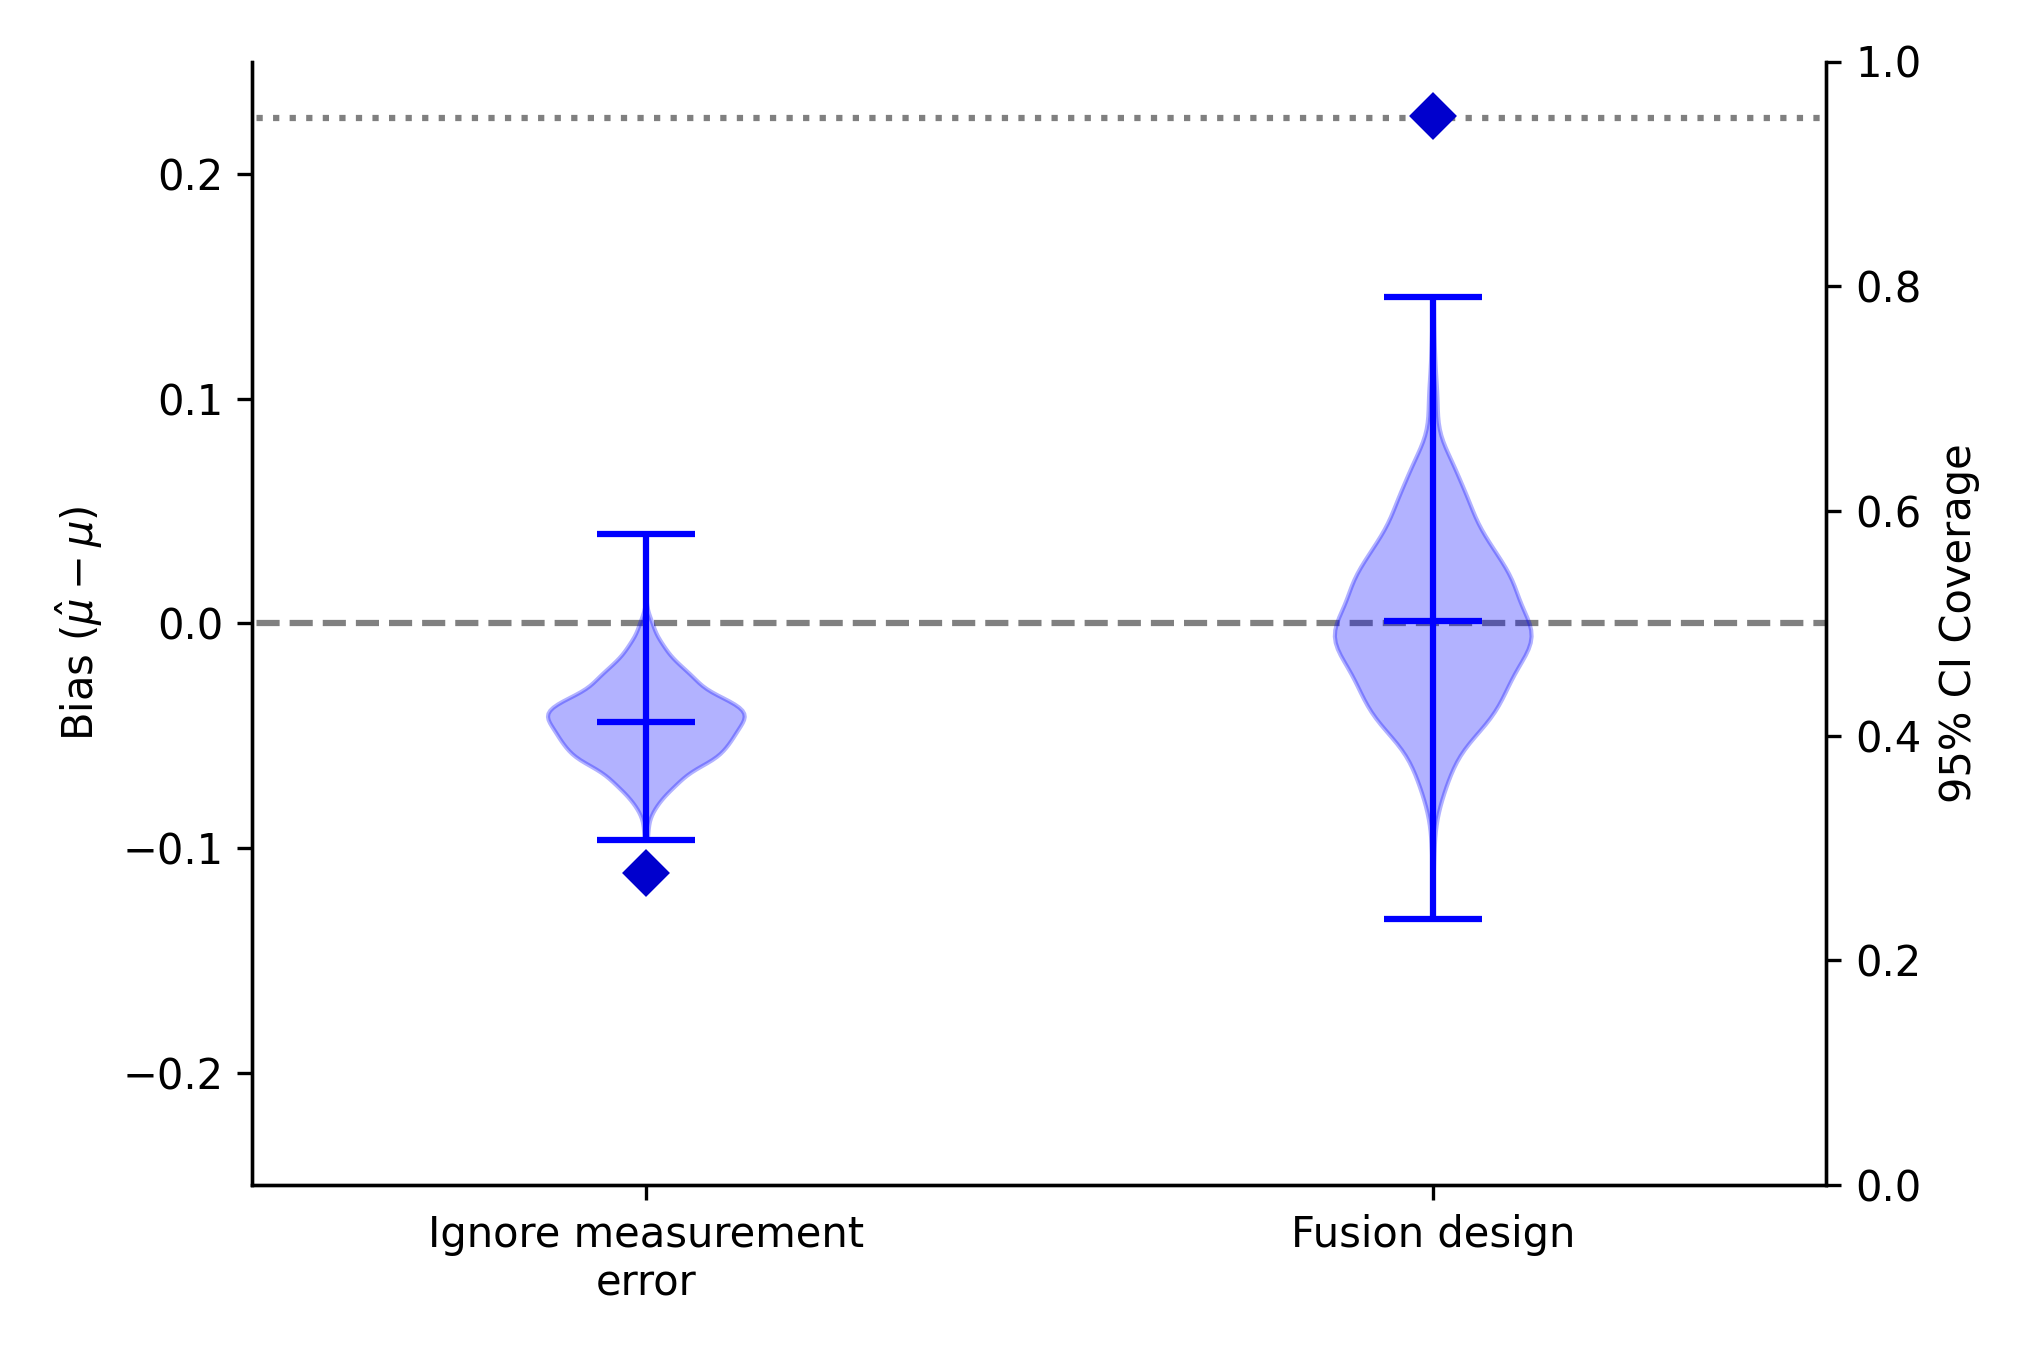
\includegraphics[scale=0.55]{images/sim_a1_results.png}
\end{frame}

\begin{frame}{A2: transport and measurement error}
	Estimate mean of variable $Y$ for population $S=3$
	\begin{center}
		\includegraphics[scale=0.55]{images/data_a2.png}
	\end{center}
\end{frame}

\begin{frame}{A2: transport and measurement error}
	Estimating functions\footnote[frame]{Measurement correction from Rogan \& Gladen (1978) \textit{Am J Epidemiol}}\textsuperscript{,}\footnote[frame]{Inverse odds weights from Westreich et al. (2017) \textit{Am J Epidemiol}}
	\[\psi(O_i; \theta) = 
	\begin{bmatrix}
		\green{I(S_i = 2) Y_i (Y_i^* - \alpha_1)} & \\
		\green{I(S_i = 2) (1-Y_i) (\left(1-Y_i^*) - \alpha_0\right)} & \\
		\violet{I(S_i \ne 2) \left( I(S_i=3) - \text{expit}(W_i^T\beta) \right) W_i} & \\
		\blue{I(S_i = 1)} \violet{\frac{1 - \text{expit}(W_i^T \beta)}{\text{expit}(W_i^T \beta)}} \blue{(Y_i^* - \omega)} & \\
		\mu(\green{\alpha_1} + \green{\alpha_0} - 1) - (\violet{\omega} + \green{\alpha_0} - 1)		
	\end{bmatrix}\]~\\
	where $O_i = (S_i, W_i, Y_i, Y_i^*)$ and $\theta = (\green{\alpha_1}, \green{\alpha_0}, \violet{\beta}, \blue{\omega}, \mu)$
\end{frame}

\begin{frame}{A2: transport and measurement error\footnote[frame]{Details and  code available at github.com/pzivich/Presentations}\textsuperscript{,}\footnote[frame]{Based on 2000 repetitions with $n_1=750$, $n_2=200$, $n_3=2000$, and $\mu=0.42$}}
	\centering 
	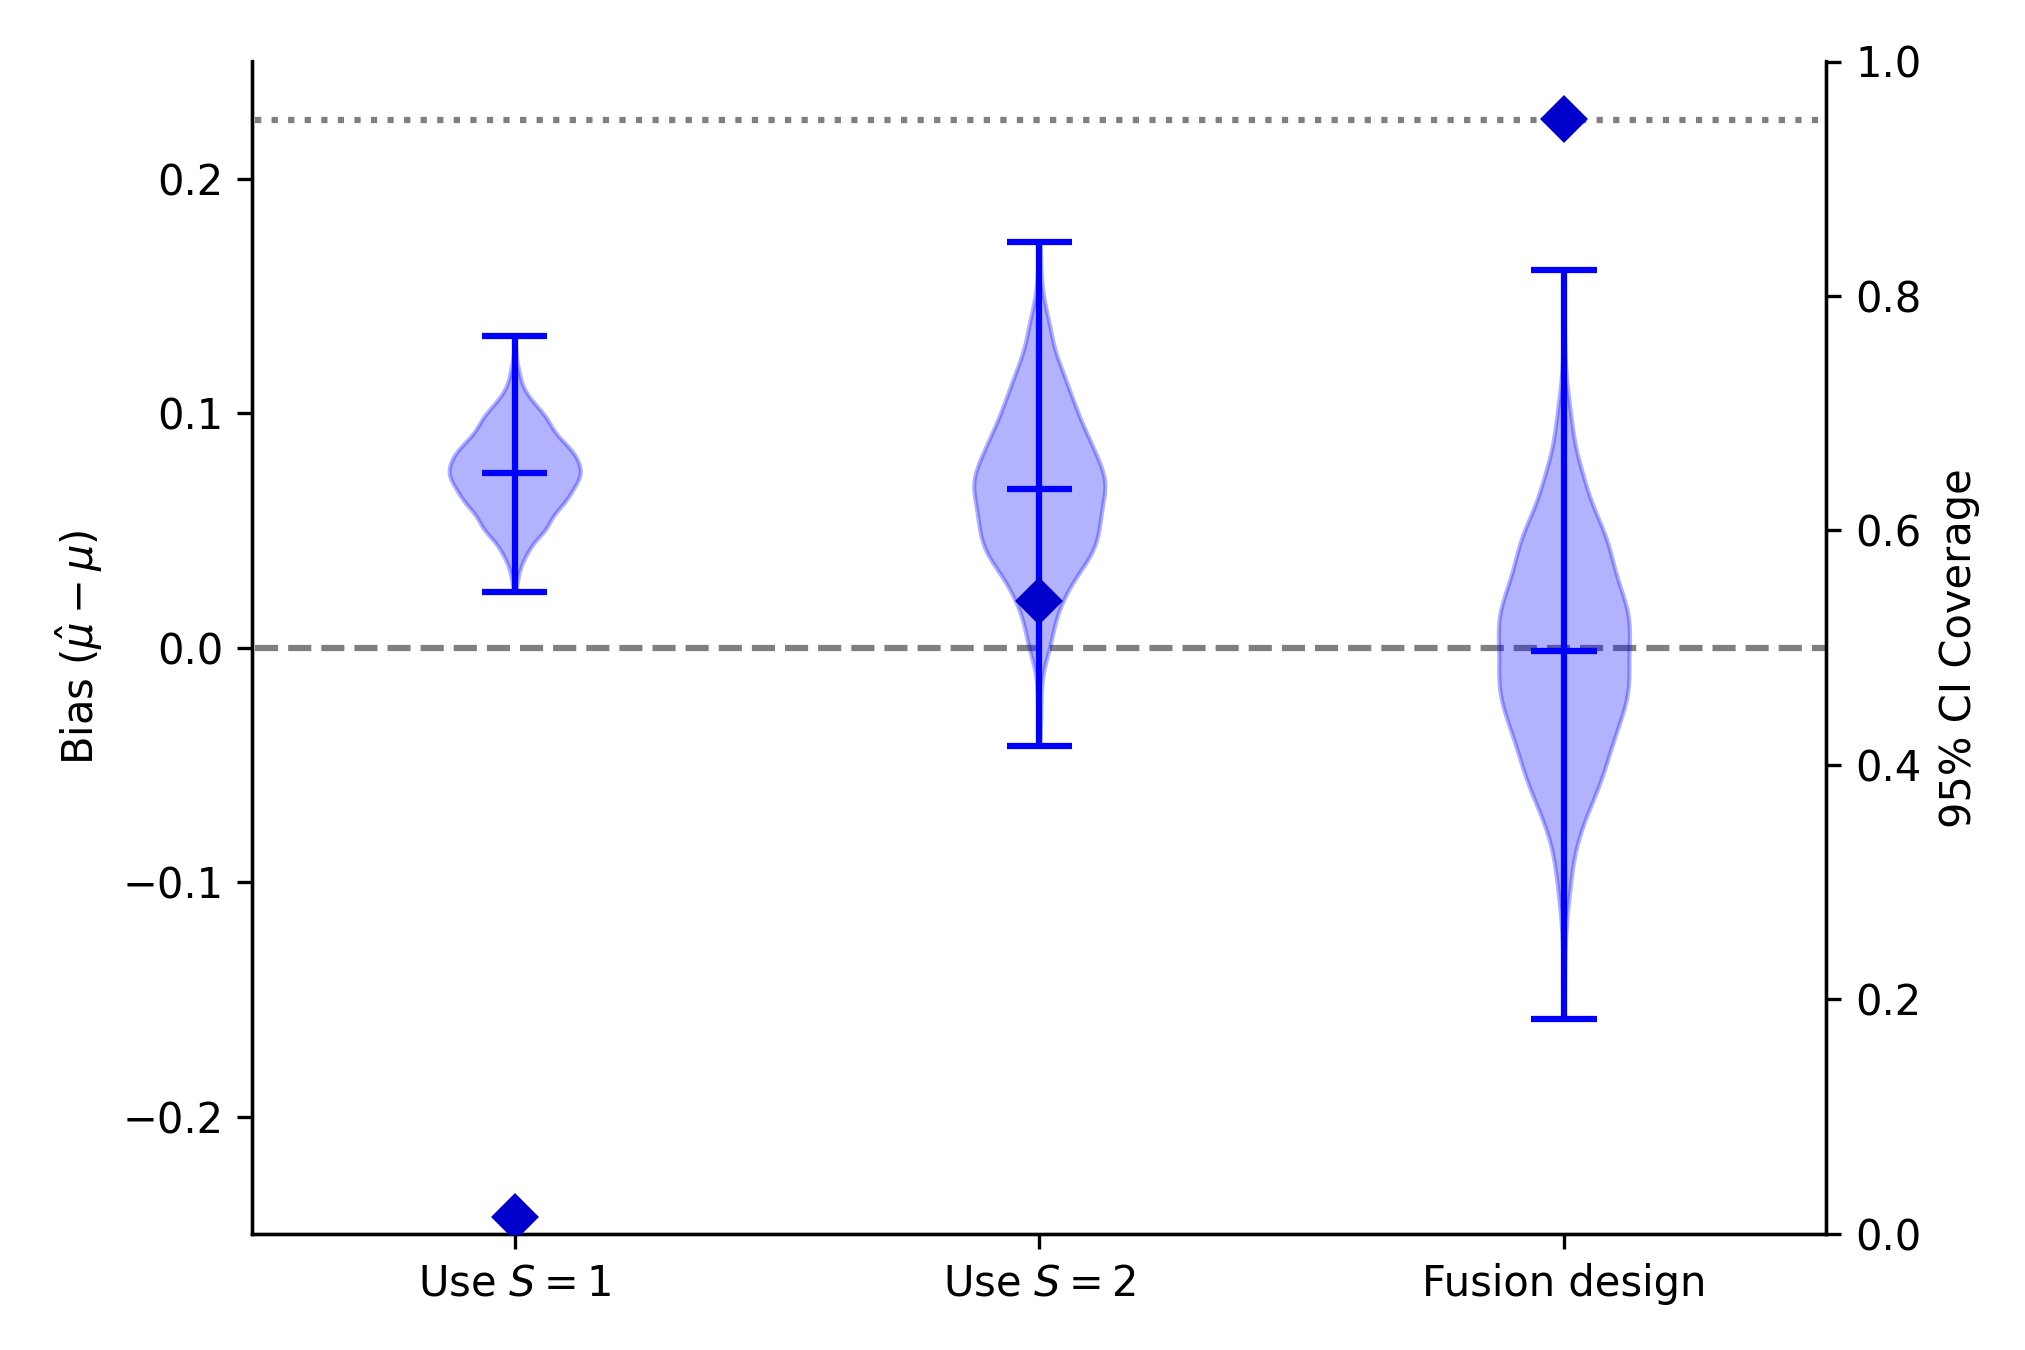
\includegraphics[scale=0.55]{images/sim_a2_results.png}
\end{frame}

\begin{frame}{A3: bridged study design}
	Compared \blue{triple therapy} to \red{mono therapy} through \violet{dual therapy}\footnote[frame]{Breskin et al. (2021) \textit{Stats in Med}}
	\begin{itemize}
		\item Using ACTG 320 and ACTG 175
		\item Restricting by CD4 between 50-300 cells/mm\textsuperscript{3}
	\end{itemize}~\\
	\[\left(\blue{F_3(t)} - \violet{F_2(t)}\right) + \left(\violet{F_2(t)} - \red{F_1(t)}\right)\]
\end{frame}

\begin{frame}{A3: bridged study design}
	Estimating functions\footnote[frame]{Here, I am using a Weibull AFT model}
	\[\psi(O_i; \theta) = 
	\begin{bmatrix}
		\left( I(S_i = 320) - \text{expit}(W_i^T) \right)W_i & \\
		I(S_i=175)\left(\red{I(A_i = 1) - \gamma_{0,1}} \right) & \\
		I(S_i=175)\left(\violet{I(A_i = 2) - \gamma_{0,2}} \right) & \\
		I(S_i=320)\left(\violet{I(A_i = 2) - \gamma_{1,2}} \right) & \\
		I(S_i=320)\left(\blue{I(A_i = 3) - \gamma_{1,3}} \right) & \\
		\psi_{AFT}(O_i; \lambda, \alpha) & \\
		\psi_{RD}(t, a; \mu_t, \beta, \gamma_{a,s}, \lambda, \alpha)
	\end{bmatrix}\]~\\
	where $O_i = (S_i, T_i^*, \delta_i, A_i, W_i)$ and $\theta = (\beta, \gamma_{a,s}, \lambda, \alpha, \mu_t)$
\end{frame}

\begin{frame}{A3: bridged study design}
	\centering 
	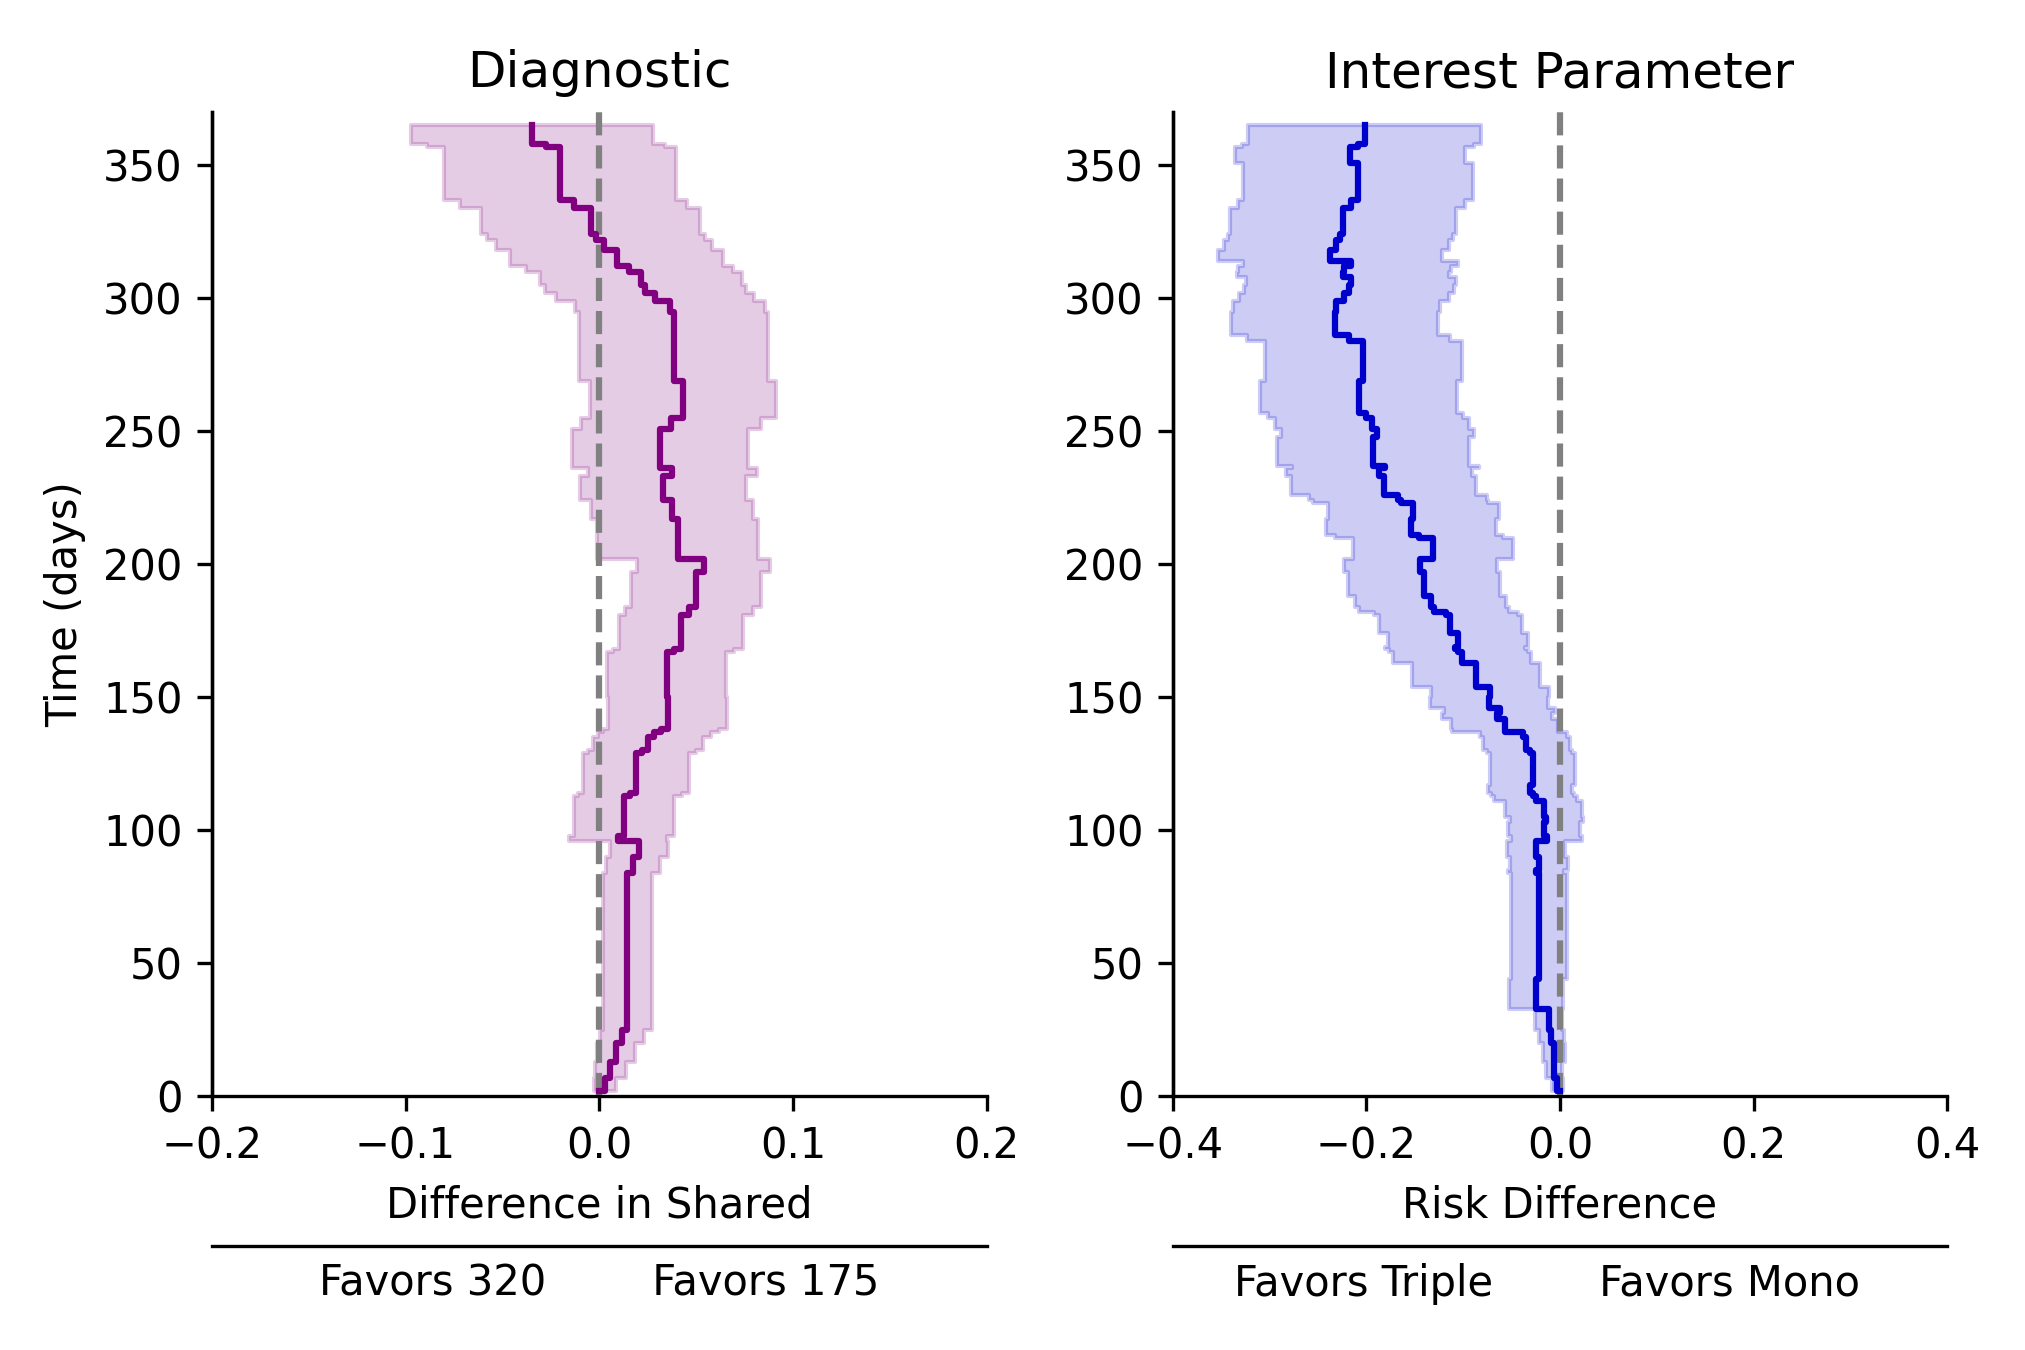
\includegraphics[scale=0.6]{images/ex_a3_results.png}
\end{frame}

\begin{frame}{Conclusion}
	M-estimation provide an adaptable way to develop fusion estimators
	\begin{itemize}
		\item Stack estimating functions together
		\item Sandwich variance estimator
	\end{itemize}~\\
	Limitations of M-estimators
	\begin{itemize}
		\item Reliance on parametric models
		\item Estimating functions can't depend on $i$
	\end{itemize}
\end{frame}

\section{Supplement}

\begin{frame}{Sandwich variance estimator}
	\[V_n(O_i; \hat{\theta}) = B_n(O_i; \hat{\theta})^{-1} F_n(O_i; \hat{\theta}) \left(B_n(O_i; \hat{\theta})^{-1}\right)^T\]~\\
	where the bread is
	\[B_n(O_i; \hat{\theta}) = \frac{1}{n} \sum_{i=1}^{n} - \psi'(O_i; \hat{\theta})\]
	and the filling is
	\[F_n(O_i; \hat{\theta}) = \frac{1}{n} \sum_{i=1}^{n} \psi(O_i; \hat{\theta}) \psi(O_i; \hat{\theta})^T\]
\end{frame}

\end{document}